This section describes the detailed implementation of SONIC in the software framework of the CMS experiment, \CMSSW; the server used to serve models, NVIDIA Triton Inference Server; and the benefits of running inference with SONIC.

\subsection{Implementation in \CMSSW}
\label{sec:implementation}

The LHC provides countercirculating beams of high energy protons, such that bunches of protons in these beams can interact with each other in the center of the CMS detector~\cite{CMS:2008xjf} every 25\unit{ns}. When protons from the countercirculating beams collide, a large variety of physical processes can occur, which then lead to the creation of either fundamental or composite particles. These particles, or their decay products, can then propagate into the CMS detector, which is designed to determine the type, energy, and momentum of each particle. Each bunch crossing where proton collisions occurs is referred to as an ``event'', in which hundreds of particles can be projected into the CMS detector. The detector itself is comprised of multiple layers including silicon pixels and strips, crystal calorimeters, sampling calorimeters, and a muon spectrometer. Each component of the detector has active components that create electrical signals when particles interact with them, either due to their charge or through interactions with the materials atomic electrons or nucleus. Each discrete signal can be called a hit.

One purpose of the \CMSSW software stack is to extract high-level physics information for each event from these hits. In essence, physicists can use \CMSSW to determine which of the large number of possible physical processes occurred in a given event, be it something relatively rare, such as the creation of a Higgs boson, or something as common the scattering of gluons in colliding protons. CMSSW processes each event with a sequence of algorithms, converting hits from electrical signals to positional and energy measurements, linking these measurements into clusters~\cite{CMS:2020uim} and trajectories~\cite{CMS:2014pgm}, combining trajectories and clusters into single particle representations and jets corresponding to hadronic showers~\cite{CMS:2017yfk}. Additional algorithms in CMS can be run to determine quantities such as the total imbalance of energy across the axis defined by the proton beam line or tag jets as containing or being produced by rare particles.

CMSSW is used both in online and offline contexts within CMS. While the Level-1 trigger is hardware-based, the high-level trigger (HLT) is constructed from algorithms in CMSSW. CMSSW also contains the algorithms that are used to process the raw data after it has been stored, deriving the higher-level information useful to physicists. The centralized offline CMS data processing flow involves two steps. The first creates an ``analysis object data'' (AOD) format derivation of every raw event, and then the second creates a slimmed, higher-level ``Mini-AOD'' derivation~\cite{Petrucciani:2015gjw}. Because algorithms within \CMSSW are occasionally modified, the raw data is reprocessed regularly. The AOD derivation step is performed twice per year and the subsequent Mini-AOD step is expected to be performed on a roughly monthly basis.

The \CMSSW framework uses Intel Threading Building Blocks~\cite{tbb} to enable task-based multithreading. As explained in Ref.~\cite{Bocci:2020olh}, this multithreading implementation allows for asynchronous non-blocking calls to external resources, such as a GPU, via ``ExternalWork''. This setup optimizes CPU resource utilization by minimizing downtime; the CPU is allowed to continue executing algorithms that do not require a coprocessor or depend on the results of the coprocessor-dependent algorithm while waiting for the external call to return.

SONIC is implemented in \CMSSW using the ExternalWork framework component, accessing coprocessor resources on remote servers via gRPC calls~\cite{gRPC}. An illustration of this procedure, where client jobs make asynchronous, non-blocking gRPC calls to a remote server, is shown in Fig.~\ref{fig:architecture}. An important aspect of this scheme is that the client-side code does not need to be able to run any particular inference packages or frameworks; it simply has to collect the relevant input data for a trained model, communicate that information to the server in the expected format, and handle the output from the server.

\begin{figure}[htp]
    \centering
    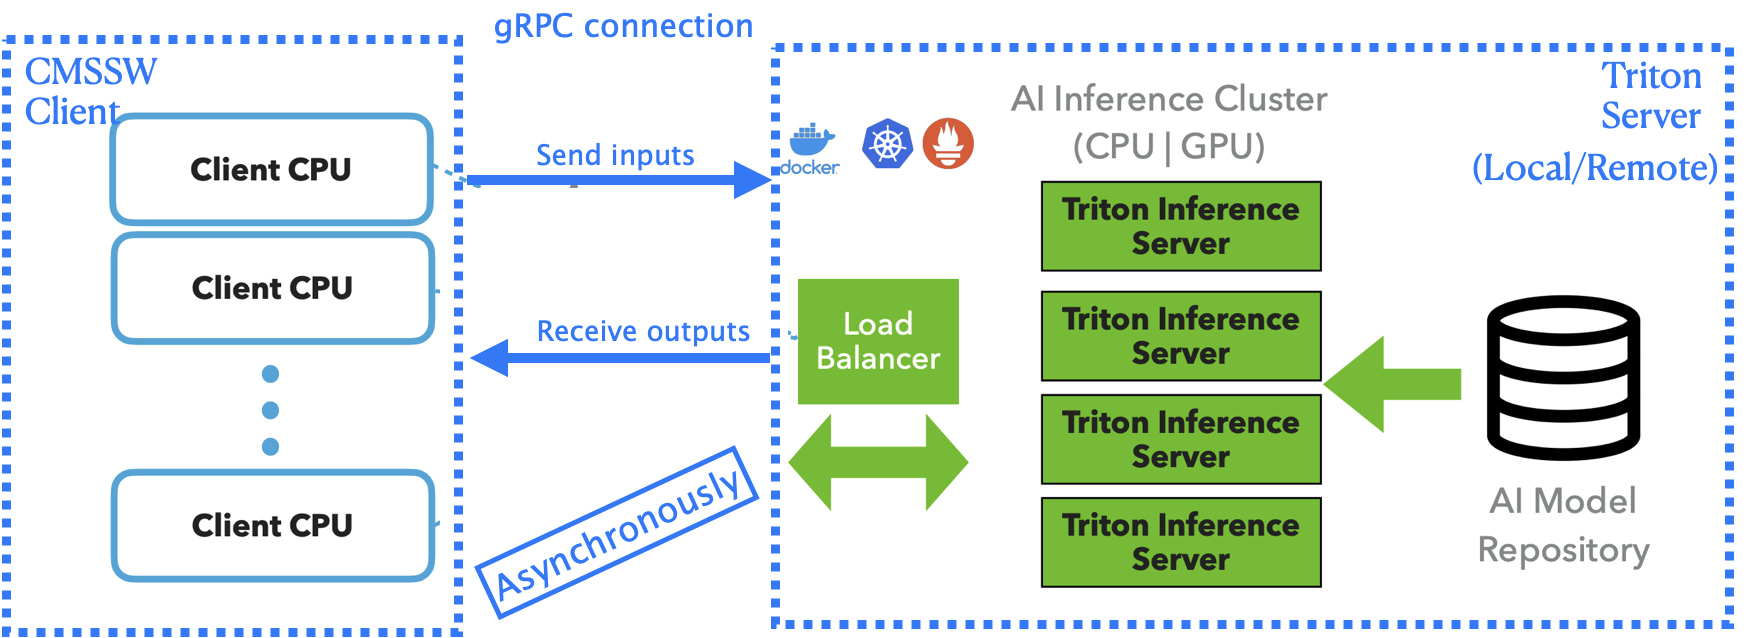
\includegraphics[width=0.90\textwidth]{plots/Architecture.png}
    \caption{Illustration of the SONIC implementation of inference as-a-service in \CMSSW. This figure also shows the possibility of an additional load-balancing layer in the SONIC scheme; for example, if multiple coprocessor-enabled machines are used to host servers, a Kubernetes engine can be set up to distribute inference calls across the machines. \textcolor{red}{(Plot will be updated to better quality)}}
    \label{fig:architecture}
\end{figure}

\subsection{NVIDIA Triton Inference Server}
\label{sec:triton}
%Document a brief introduction about the NVIDIA Triton inference server

As shown in Fig.~\ref{fig:architecture}, the GPU-based implementation of SONIC in \CMSSW uses the NVIDIA Triton Inference Server to deploy ML inference on the coprocessors~\cite{triton, triton_readme}. Triton servers can perform inference for ML algorithms, or ``models'', in most modern formats, including \PYTORCH, TensorRT, ONNX Runtime, \TENSORFLOW, and \XGBOOST, and also supports custom backends for alternative tasks. A single server can host multiple models at the same time or even multiple instances of the same model to allow concurrent inference requests. Triton also supports dynamic batching: if multiple inference calls are made within a window of time, the server can concatenate all calls' inputs into a single batch, which improves the GPU utilization and therefore increases the overall throughput. Parameters such as the number of model instances on a single server, the length of a batching window, and the optimal batch size are tunable and can be optimized on a case-by-case basis. Triton provides a model analyzer tool to aid in this optimization~\cite{triton_model_analyzer}.

Triton servers can use one or multiple GPUs on the same machine with a built-in load balancer. Triton servers can also run purely on CPU resources when there are no GPU resources available. For other types of coprocessors, Triton servers can also be used with the help of custom backends. To start a server, it is only necessary to provide a trained model file and sometimes a configuration file specifying input and output variable names, shapes, types, and model versions. Client-side jobs are configured with servers' address and port numbers in order to carry out communications, and jobs must provide input with the correct format for inference.

It is important to note that Triton provides an open source solution for implementing IaaS, with a public set of protocols. It is also possible to use those protocols in alternative server implementations, as was done in the FPGAs-as-a-Service Toolkit~\cite{FaaST}.%not strictly necessary to use Triton's set of protocols; for example, server protocols were independently reimplemented for communication with inference servers in the FPGAs-as-a-Service Toolkit~\cite{FaaST}.

\subsection{Advantages of SONIC}
\label{sec:sonic_benefits}
While many of the benefits of running with SONIC have been mentioned throughout the preceding text, it is worthwhile to quickly summarize some of these points here.
\begin{itemize}
    \item \emph{Containerization}: SONIC factorizes ML frameworks out of the client software stack, i.e., \CMSSW, making it easier support a wide variety of ML models. Currently, any ML algorithms in \CMSSW must either be cast in one of a limited number of supported frameworks, or else support for a new framework must be added. With SONIC, one can use any framework supported by Triton, including custom backends, with no modification of \CMSSW needed. This allows physicists to pick the best ML inference backend with less concern for the implementation details. This ``support'' for a wide variety of frameworks is easy to maintain.
    \item \emph{Simplicity}: Because of the containerization discussed above, client-side code that takes advantage of SONIC can be simplified. Generic functions for sending input to and receiving output from servers can be defined, and then to deploy any model deployed in the workflow, client code only needs to format model inputs correctly and collect the outputs.
    \item \emph{Flexibility}: In the SONIC paradigm, the ratio of CPU resources to GPU resources is not fixed, as clients from many different machines can access a single server running on either one GPU or multiple GPUs. Similarly, a single client can access multiple different servers running on multiple different machines. GPU-to-CPU ratios can therefore be adjusted for different ML inference tasks, allowing optimal utilization of coprocessor resources.
    \item \emph{Efficiency}: SONIC enables superior utilization of coprocessor resources. By optimizing the GPU-to-CPU ratio, it is easier to come close to saturating GPU resources without oversaturating them. Because of this, any GPU purchase can be kept to the minimal number of GPUs necessary, saving overall cost.
    \item \emph{Portability}: Through the use of SONIC, client-side workflows do not have to be modified to take advantage of different types of coprocessors. As long as a consistent protocol exists for communicating with the inference server, it does not matter if the server is on a CPU, GPU, FPGA, IPU, or any other architecture. This allows users to easily take advantage of whatever resources are available and easily optimize workflows if there are multiple options.
    \item \emph{Accessibility}: It is worth explicitly pointing out that SONIC is the only way for any CPU to access remote GPUs or other coprocessors. This should reduce costs associated with coprocessor-based inference acceleration, allowing for collaborators to share resources more easily. While calls to a remote server introduce a distance-dependent latency, the use of asynchronous calls in SONIC means that the overall event latency is negligibly impacted~\cite{Krupa:2020bwg}. SONIC can also use local resources if they are available.
\end{itemize}

It is also important to point out that within CMSSW, a mechanism has been implemented to account for the possibility that a client job cannot access a specified server for whatever reason. In this case, a ``fallback'' server is automatically created using either GPU resources if they are available or the CPU resources allocated to the client job in question. The client then makes gRPC calls to that local fallback server, which introduces negligible latency. The server overhead generally consumes very little of the CPU resources beyond what would be used for conventional inference, such that the per-event latency is not strongly affected by SONIC relative to running without SONIC. Fallback servers are automatically shut down when the job finishes. Studies related to these fallback servers are discussed in Section~\ref{sec:fallback}.
